\documentclass[tikz,border=14pt]{standalone}
\usepackage[T1]{fontenc}
\usepackage{helvet}
\renewcommand{\familydefault}{\sfdefault}
\usepackage{xcolor}
\usetikzlibrary{shapes.multipart,arrows.meta,calc}

\definecolor{role}{HTML}{1F5FA8}

\tikzset{
  base/.style={font=\footnotesize, inner xsep=5pt, inner ysep=3pt, line width=0.7pt,
               draw=black, fill=white, align=left},
  cls/.style={base, rectangle split, rectangle split parts=2, text width=#1},
  cls3/.style={base, rectangle split, rectangle split parts=3, text width=#1},
  cls0/.style={base, rectangle, text width=#1, align=center},
  gen/.style ={line width=0.7pt, -{Triangle[open, length=7pt, width=7pt]}},
  real/.style={line width=0.7pt, dashed, -{Triangle[open, length=7pt, width=7pt]}},
  dep/.style ={line width=0.7pt, dashed, -{Stealth[length=6pt, width=5pt]}},
  ass/.style ={line width=0.7pt, -{Stealth[length=6pt, width=5pt]}},
  agg/.style ={line width=0.7pt, {Diamond[open, length=9pt, width=6pt]}-{Stealth[length=6pt, width=5pt]}},
  lbl/.style ={font=\scriptsize\itshape, fill=white, inner sep=1.5pt},
  role/.style={font=\scriptsize\bfseries\itshape, text=role, inner sep=2pt, anchor=south east},
  note/.style={font=\scriptsize, draw=black!70, dashed, fill=black!4, inner sep=4pt, align=left},
}
\newcommand{\hd}[2]{{\centering\scriptsize\itshape #1\par}{\centering\bfseries #2\par}}

\begin{document}
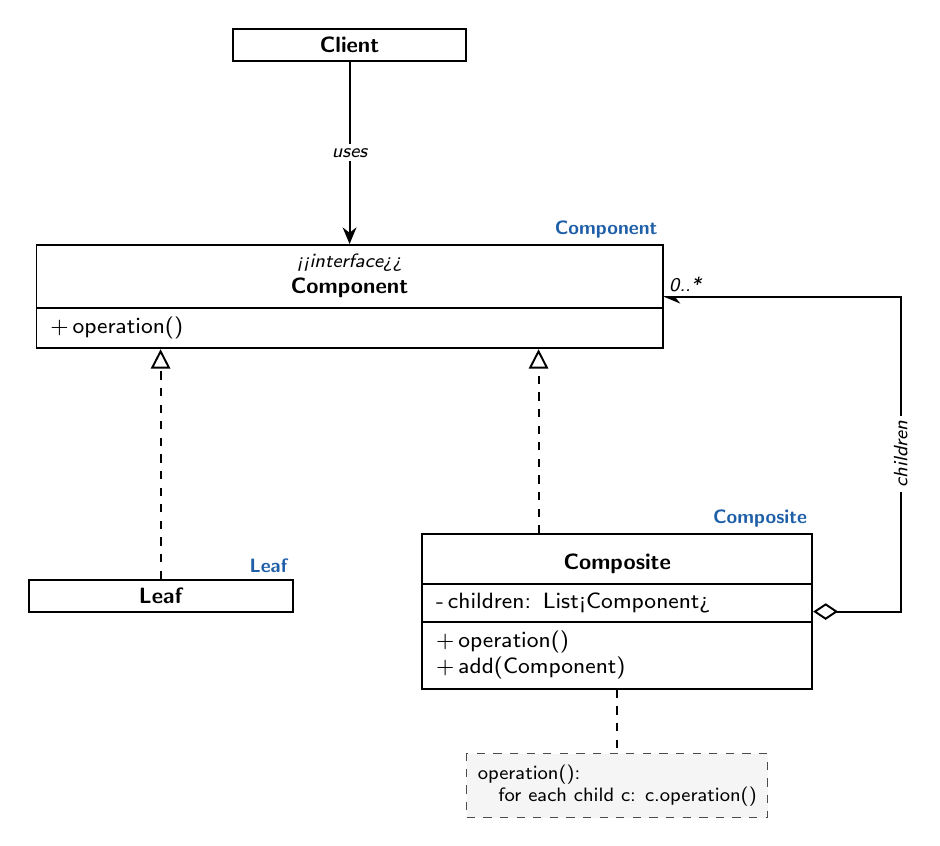
\begin{tikzpicture}

% ---------- nodes (example: Composite) ----------
\node[cls0=2.6cm] (Client) at (5,0) {\bfseries Client};

\node[cls=7.6cm] (Comp) at (5,-3.2) {\hd{<<interface>>}{Component}
  \nodepart{second}+\,operation()};

\node[cls0=3.0cm] (Leaf) at (2.6,-7.0) {\bfseries Leaf};

\node[cls3=4.6cm] (Cmp) at (8.4,-7.2) {\hd{}{Composite}
  \nodepart{second}-\,children: List<Component>
  \nodepart{third}+\,operation()\\
  +\,add(Component)};

\node[role] at (Comp.north east) {Component};
\node[role] at (Leaf.north east) {Leaf};
\node[role] at (Cmp.north east)  {Composite};

% ---------- edges ----------
\draw[ass] (Client.south) -- (Comp.north) node[lbl, midway] {uses};
\draw[real] (Leaf.north) -- (Leaf.north |- Comp.south);
\draw[real] (7.4,0 |- Cmp.north) -- (7.4,0 |- Comp.south);
\draw[agg] (Cmp.east) -- (12.0,-7.2) -- (12.0,-3.2) -- (Comp.east);
\node[lbl, anchor=south west] at (9.0,-3.2) {0..*};
\node[lbl, rotate=90] at (12.0,-5.2) {children};

\node[note, anchor=north] (N) at (8.4,-9.0) {operation():\\\hspace*{1em}for each child c: c.operation()};
\draw[dashed, line width=0.6pt] (Cmp.south) -- (N.north);

\end{tikzpicture}
\end{document}
